% =====================================================================
%  Mid-Semester Project Report  --  IEEE double-column format (4 pages)
%  Compile with pdflatex (e.g. upload this folder to Overleaf).
%  Fill in every [[ ... ]] placeholder before printing.
% =====================================================================
\documentclass[conference]{IEEEtran}
\IEEEoverridecommandlockouts
\usepackage{cite}
\usepackage{amsmath,amssymb}
\usepackage{graphicx}
\usepackage{booktabs}
\usepackage{array}
\usepackage{xcolor}
\usepackage{tikz}
\usetikzlibrary{positioning,arrows.meta,calc}
\graphicspath{{figures/}}

\newcommand{\R}{\mathbb{R}}

% ---- drawing helpers for the architecture figure (CRA-Net-paper style) ----
% stacked feature maps: {size in mm}{fill}{draw}
\tikzset{pics/fmap/.style n args={3}{code={%
  \foreach \k in {1,2,3}{%
    \filldraw[draw=#3, fill=#2, line width=0.5pt]
      ({(\k-2)*1.4-#1/2},{-(\k-2)*1.4-#1/2}) rectangle ++(#1,#1);}%
  \draw[densely dashed, rounded corners=2pt, black!65]
      ({-#1/2-3.4},{-#1/2-3.4}) rectangle ({#1/2+3.4},{#1/2+3.4});}}}
% operation bar: {x}{y}{height}{colour}
\newcommand{\opbar}[4]{%
  \shadedraw[top color=#4!20, bottom color=#4!65, draw=#4!70!black]
    ({#1-1.5},{#2-#3/2}) rectangle ({#1+1.5},{#2+#3/2});}

\begin{document}

\title{AnatoPhaseNet: Phase-Aligned Anatomical Spatio-Temporal Network for
Subject-Independent Pathological Gait Classification from Silhouettes}

\author{
\IEEEauthorblockN{[[Student Name 1]] ([[Roll No.]]), [[Student Name 2]] ([[Roll No.]])}
\IEEEauthorblockA{Department of [[Department]], [[Institute]]\\
Supervisor: [[Supervisor Name]]}
}

\maketitle

\begin{abstract}
Video-based pathological gait classification can support low-cost
screening, but a useful model must work on people it has never seen. We
classify side-view silhouettes from GAIT-IT and INIT and evaluate every model
with 10-fold subject-exclusive cross-validation. Starting from a frame-level
attention network, we went through nine stages to AnatoPhaseNet, which aligns
each gait cycle to nine clinical phases, encodes it with an ImageNet-inflated
(2+1)D ResNet-18 with circular temporal convolutions, pools six body strips with
a half-cycle symmetry descriptor, and adds a posture-geometry branch and a
multi-cycle walk head. With 5.0\,M parameters it
reaches 95.47\,\% cycle and 96.28\,\% walk accuracy on GAIT-IT and 92--93\,\%
on INIT (6 classes), on unseen subjects only.
\end{abstract}

\begin{IEEEkeywords}
Pathological gait, silhouettes, (2+1)D CNN, gait phases, subject-independent
evaluation, GAIT-IT, INIT.
\end{IEEEkeywords}

% =====================================================================
\section{Introduction}
% =====================================================================
Gait depends on the coordination of muscles, joints and the nervous system, so
Parkinson's disease, cerebral palsy (diplegia), stroke (hemiplegia) and
peripheral neuropathy each leave a characteristic walking
pattern~\cite{baker2018}. Marker-based gait labs are expensive; a single
side-view camera with silhouette extraction is cheap and privacy-preserving.

\textbf{Motivation.} In a diagnostic setting the model always meets a
\emph{new} patient. If images of the same person appear in training and test,
a network can recognise the person instead of the pathology. We therefore
test only on unseen subjects and base each part of the model on gait
biomechanics (phases, body parts, symmetry, posture).

\textbf{Data and protocol.} GAIT-IT~\cite{albuquerque2021}: 23 subjects, 821
annotated sequences (3813 gait cycles), five gait types (normal, diplegic, hemiplegic, neuropathic,
Parkinsonian), each at two levels. INIT~\cite{ortells2018}: 10 subjects, 160
sequences, eight styles (normal, reduced left/right arm swing at two levels,
half left/right leg step, full-body impairment); the 6-class protocol merges
the two arm levels. Fold $k$ tests on subject group $k$, monitors training on
group $k{+}1$ and trains on the rest, with a fixed seed, so all models are
tested on the same people. We train for a fixed 20 epochs and test the final
weights, so the test subjects influence no choice.

\textbf{Objectives.} (1) Classify a gait cycle of an unseen subject; (2) give a
walk-level decision; (3) train on a 4\,GB laptop GPU.

% =====================================================================
\section{Literature Review}
% =====================================================================
\textbf{Energy images.} Early silhouette methods compress a walk into one image.
Verlekar \emph{et al.}~\cite{verlekar2018} classified Gait Energy Images (GEI)
with a fine-tuned VGG-19. Albuquerque \emph{et al.}~\cite{albuquerque2021}
released GAIT-IT and reached 94.0\,\% with VGG-19 on GEIs under a
subject-independent protocol. Averaging over time, however, discards the order
of the gait phases.

\textbf{Attention CNNs.} SE~\cite{hu2018se}, CBAM~\cite{woo2018cbam} and
non-local blocks~\cite{wang2018nonlocal} re-weight channels and positions of a
frame. CRA-Net~\cite{bodepu_cranet} combines an encoder--decoder with reverse
cross-attention fusion in 0.93\,M parameters; it classifies frames one at a
time and does not state a subject-exclusive split, so we used it only as our
starting point.

\textbf{Temporal and part models.} I3D~\cite{carreira2017i3d} inflates
ImageNet 2D filters into 3D; (2+1)D convolutions~\cite{tran2018r21d} factorise a
3D kernel into spatial and temporal parts; TSM~\cite{lin2019tsm} shifts channels
in time at no parameter cost; SSAN~\cite{guo2021ssan} separates spatial and
temporal self-attention. For gait recognition, GaitSet~\cite{chao2019gaitset}
pools horizontal body strips and TransGait~\cite{li2023transgait} uses vision
transformers.

\textbf{Gap.} Frame-level and energy-image methods ignore that walking is
periodic, and part-based gait models target identity, not pathology. No prior
model combines phase alignment, part-level temporal features, symmetry and
posture geometry under a subject-exclusive protocol.

% =====================================================================
\section{Experimental Journey}
% =====================================================================
Table~\ref{tab:journey} lists everything we tried, in order. Each stage was
started by a failure observed in the previous one.

\begin{table*}[!t]
\centering
\caption{What we tried, why, and what we learned (GAIT-IT accuracies are on unseen subjects unless marked)}
\label{tab:journey}
\footnotesize
\setlength{\tabcolsep}{3pt}
\begin{tabular}{@{}p{0.5cm}p{2.6cm}p{6.4cm}p{3.6cm}p{3.8cm}@{}}
\toprule
Stage & Model & What we built & Why & Outcome \\
\midrule
1 & ST-CRA-Net (6.59\,M) & CRA-Net~\cite{bodepu_cranet} extended to 12 uniform frames; axial, harmonic temporal attention; temporal reverse-attention pooling & Start from CRA-Net; walking is a movement, not an image & 100\,\% train, 77.24\,\% val: memorises people \\
2 & Swin (7.81\,M) & CRA-Net frame classifier with its conv encoders replaced by Swin blocks~\cite{liu2021swin} & Test whether stronger attention helps & $\approx$93\,\% val, but frame-level with shared subjects; no motion \\
3 & Compact (2+1)D & (2+1)D convs, motion channel, augmentation, EMA & Smaller model & 87.96\,\% val; gap 23$\rightarrow$7 points \\
4 & Protocol fix & Split by person ID (23, not 114 groups); 10 fixed folds & One person performs all five gaits & Honest folds for all later models \\
5 & ST-PhaseNet & One sample = one gait cycle at its 9 clinical key frames & Uniform sampling mixes phases & \textbf{89.10\,\%} cycle \\
6 & + Regions, crop, focal & Upper/lower body regions; bounding-box crop to $96^2$; focal loss & Diseases affect different body parts & 91.08 / \textbf{93.34} / 93.01\,\% \\
7 & + Defect fixes & Direction canonicalisation, ImageNet inflation, circular time conv, 6 strips, symmetry, part ensemble & Train 99.96\,\%: generalisation problem & \textbf{94.05\,\%}, fold std $5.38\rightarrow4.04$ \\
8 & + Walk head & Multi-cycle stride-variability head & Variability is a clinical marker & \textbf{95.71\,\%} walk \\
9 & + Geometry (final) & Posture-geometry branch & Cropping hides crouch, stoop, bob & \textbf{95.47\,\%} cycle, \textbf{96.28\,\%} walk \\
\bottomrule
\end{tabular}
\end{table*}

Two lessons shaped the design. \emph{Phase alignment:} for a walk at speed
$\alpha$, $x_\alpha(t)=x(\alpha t)$, so sampling at the phase events gives
$x_\alpha(\tau_p/\alpha)=x(\tau_p)$ --- the same nine inputs at any cadence, and
$4.6\times$ more samples (3813 cycles). \emph{Audit before adding:} stage-7
gains came from fixing defects (e.g.\ back walks mirror front walks:
correlation 0.65 raw, 0.996 after a flip), not from a bigger network.

% =====================================================================
\section{Final Architecture: What Each Block Does}\label{sec:arch}
% =====================================================================
\begin{figure*}[!t]
\centering
\resizebox{\textwidth}{!}{%
\begin{tikzpicture}[x=1mm, y=1mm,
  lbl/.style={font=\tiny, align=center, inner sep=0.5pt, anchor=north},
  ttl/.style={font=\scriptsize\itshape, anchor=north west, inner sep=1pt},
  arr/.style={-{Stealth[length=1.5mm]}, semithick},
  pnl/.style={draw=black!45, dash dot, rounded corners=5pt, fill=white!92!yellow},
  op/.style={circle, draw, thick, minimum size=6mm, inner sep=0pt, font=\scriptsize, fill=white},
  outb/.style={draw, rounded corners=2pt, fill=black!8, font=\scriptsize\bfseries,
               align=center, minimum height=7mm, text width=15mm},
  mini/.style={draw, rounded corners=1.5pt, fill=white, font=\tiny, align=center,
               inner sep=1pt, text width=11mm}]
% =================== overall model ===================
\fill[yellow!12, rounded corners=3pt] (0,2) rectangle (184,-86);
\draw[black!60, rounded corners=3pt] (0,2) rectangle (184,-86);
\draw[pnl] (27,0) rectangle (148,-29.5);
\draw[pnl] (27,-32) rectangle (148,-55);
\draw[pnl] (27,-58) rectangle (148,-84);
\node[ttl] at (28,-0.3) {Appearance stream (B3--B5)};
\node[ttl] at (28,-32.3) {Geometry stream (B6) and descriptor $g$};
\node[ttl] at (28,-58.3) {Walk head (B8)};
% ---- input (B1, B2)
\node at (13,-27) {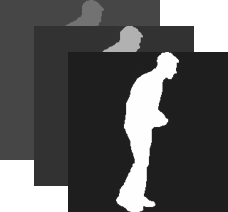
\includegraphics[width=22mm]{phase_stack.png}};
\node[lbl] at (13,-39.5) {\textbf{B1--B2}: gait cycle,\\9 clinical phases,\\crop $3{\times}96^2$};
\draw[arr] (24.5,-20) -- (28.3,-13);
\draw[arr] (24.5,-33) -- (31,-41) node[midway, right, font=\tiny] {raw};
% ---- row 1: appearance stream (centre y = -13)
\pic at (37,-13) {fmap={10}{cyan!35}{blue!60!black}};
\opbar{49.5}{-13}{14}{blue}
\pic at (59,-13) {fmap={9}{cyan!35}{blue!60!black}};
\opbar{70}{-13}{12}{blue}
\pic at (79,-13) {fmap={7.5}{cyan!35}{blue!60!black}};
\opbar{89}{-13}{10}{blue}
\pic at (97,-13) {fmap={6}{cyan!35}{blue!60!black}};
\foreach \i in {0,...,5}{%
  \filldraw[draw=orange!70!black, fill=orange!18] (107,{-6.4-\i*2.2}) rectangle (115,{-6.4-(\i+1)*2.2});}
\filldraw[draw=black!60, fill=black!12] (116.3,-6.4) rectangle (118.3,-19.6);
\opbar{122.5}{-13}{14}{orange}
\foreach \i in {0,...,6}{%
  \filldraw[draw=violet!70!black, fill=violet!15] ({126+\i*1.6},-7) rectangle ({127.2+\i*1.6},-19);}
\opbar{143}{-13}{14}{violet}
\node[lbl] at (37,-22.6) {Stem\\$64{\times}9{\times}24^2$};
\node[lbl] at (59,-22.6) {Layer 1\\$64{\times}9{\times}24^2$};
\node[lbl] at (79,-22.6) {Layer 2\\$128{\times}9{\times}12^2$};
\node[lbl] at (97,-22.6) {Layer 3\\$256{\times}9{\times}6^2$};
\node[lbl] at (112.7,-21.2) {\textbf{B4}: 6 strips\\+ global};
\node[lbl] at (122.5,-21.2) {phase emb.\\circ.\ conv};
\node[lbl, anchor=south] at (131.5,-6.4) {\textbf{(b)} \textbf{B5}: $7{\times}384$};
\node[lbl] at (143,-21.2) {7 part\\classifiers};
\node[font=\tiny\bfseries, text=brown!80!black] at (88,-2.8) {(a) B3 blocks, ImageNet-inflated};
\draw[arr] (45.5,-13) -- (48,-13);  \draw[arr] (66.9,-13) -- (68.5,-13);
\draw[arr] (86.1,-13) -- (87.5,-13); \draw[arr] (103.4,-13) -- (106.8,-13);
\draw[arr] (118.5,-13) -- (121,-13); \draw[arr] (124,-13) -- (125.8,-13);
\draw[arr] (137.3,-13) -- (141.5,-13);
% ---- row 2: geometry stream (centre y = -42)
\draw[-{Stealth[length=1mm]}] (32,-47) -- (47,-47);
\draw[-{Stealth[length=1mm]}] (32,-47) -- (32,-36);
\draw[blue!70, thick] plot[domain=0:13, smooth, samples=40] ({33+\x},{-41.5+2.5*sin(\x*55)});
\draw[red!70, thick] plot[domain=0:13, smooth, samples=40] ({33+\x},{-43+1.8*cos(\x*55)});
\draw[green!50!black, thick] plot[domain=0:13, smooth, samples=40] ({33+\x},{-45+1*sin(\x*110)});
\opbar{57}{-42}{12}{orange}
\opbar{63}{-42}{12}{orange}
\foreach \i in {0,...,2}{%
  \filldraw[draw=green!45!black, fill=green!20] ({72+\i*2.4},-37) rectangle ({73.8+\i*2.4},-47);}
\node[op] (g) at (106,-40) {$g$};
\opbar{143}{-42}{12}{violet}
\node[lbl] at (39.5,-48.3) {\textbf{B6}: 9 signals on the raw\\silhouette ($\div$ median height)};
\node[lbl] at (60,-48.3) {2 circular\\temporal convs};
\node[lbl] at (76,-48.3) {mean$\Vert$max$\Vert$sym\\192-d};
\node[lbl, anchor=west] at (109.4,-40) {descriptor\\2880-d};
\node[lbl] at (143,-48.3) {geometry\\classifier};
\draw[arr] (47.5,-42) -- (55.5,-42); \draw[arr] (58.5,-42) -- (61.5,-42);
\draw[arr] (64.5,-42) -- (71.8,-42);
\draw[arr] (79.3,-40) -- (103,-40);
\draw[arr] (79.3,-45.5) -- (141.5,-45.5);
\draw[arr] (131.5,-19.3) -- (131.5,-30.7) -| (106,-37);
% ---- B7: average of the 8 classifiers -> cycle class
\node[op] (avg) at (156,-27) {avg};
\node[font=\tiny\bfseries, anchor=east] at (152.7,-27) {B7};
\draw[arr] (144.5,-13) -| (avg.north);
\draw[arr] (144.5,-42) -| (avg.south);
\node[outb] (o1) at (174,-27) {Cycle\\class};
\draw[arr] (avg) -- (o1);
% ---- row 3: clinical heads (centre y = -69)
\node at (37,-69) {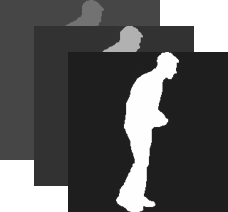
\includegraphics[width=10mm]{phase_stack.png}};
\opbar{50}{-69}{12}{gray}
\pic at (62,-69) {fmap={5}{green!25}{green!45!black}};
\node[font=\scriptsize] (stats) at (80,-69) {$[\boldsymbol\mu\Vert\boldsymbol\sigma\Vert\boldsymbol\delta]$};
\opbar{95}{-69}{12}{magenta}
\node[lbl] at (37,-75.7) {$K{=}2..6$ cycles\\of one walk};
\node[lbl] at (50,-75.7) {B2--B5\\shared};
\node[lbl] at (62,-75.7) {$\mathbf{e}_k\in\R^{256}$};
\node[lbl] at (80,-75.7) {mean, std, successive\\difference (variability)};
\node[lbl] at (95,-75.7) {\textbf{B8}: walk\\classifier};
\draw[arr] (42.5,-69) -- (48.5,-69); \draw[arr] (51.5,-69) -- (56,-69);
\draw[arr] (68,-69) -- (stats.west); \draw[arr] (stats.east) -- (93.5,-69);
\draw[semithick] (106,-43) -- (106,-60.5);
\draw[arr] (106,-60.5) -| (62,-64.4);
\node[font=\tiny, anchor=south] at (84,-60.5) {$\mathbf{e}_k=\mathrm{MLP}(g_k)$};
\node[outb] (o3) at (174,-69) {Walk\\class};
\draw[arr] (96.5,-69) -- (166.5,-69);
% =================== (a) inflated (2+1)D block ===================
\draw[draw=brown!70!black, densely dashed, rounded corners=6pt, fill=yellow!28] (0,-89) rectangle (86,-123);
\node[ttl] at (1.5,-89.5) {(a) One (2+1)D block of layers 1--3 (B3)};
\pic at (8,-102) {fmap={4}{cyan!35}{blue!60!black}};
\opbar{20}{-102}{12}{cyan}
\opbar{32}{-102}{12}{orange}
\node[op, minimum size=4.5mm] (p1) at (43,-102) {$+$};
\opbar{54}{-102}{12}{cyan}
\node[op, minimum size=4.5mm] (p2) at (65,-102) {$+$};
\pic at (77,-102) {fmap={4}{cyan!35}{blue!60!black}};
\draw[arr] (13.5,-102) -- (18.5,-102); \draw[arr] (21.5,-102) -- (30.5,-102);
\draw[arr] (33.5,-102) -- (p1); \draw[arr] (p1) -- (52.5,-102);
\draw[arr] (55.5,-102) -- (p2); \draw[arr] (p2) -- (71.5,-102);
\draw[arr] (25.5,-102) -- (25.5,-95.2) -| (p1.north);
\draw[arr] (8,-96.6) -- (8,-93.8) -| (p2.north);
\node[lbl] at (8,-108.5) {$\mathbf{x}$};
\node[lbl] at (20,-108.5) {$1{\times}3{\times}3$ conv\\(ImageNet)};
\node[lbl] at (32,-108.5) {$3{\times}1{\times}1$\\circular conv};
\node[lbl] at (43,-108.5) {$\mathbf{u}{+}\mathrm{BN}_t(\cdot)$};
\node[lbl] at (54,-108.5) {$1{\times}3{\times}3$ conv\\(ImageNet)};
\node[lbl] at (65,-108.5) {skip};
\node[lbl] at (77,-108.5) {$\mathbf{y}$};
\node[font=\tiny, align=left, text width=82mm, anchor=north west] at (2,-114) {Phase 9 wraps to phase 1 (circular padding: no phase is an edge).
$\mathrm{BN}_t$ starts at $\gamma{=}0$, so at step 0 the block is exactly the pretrained 2D ResNet block.};
% =================== (b) part temporal head ===================
\draw[draw=red!60!black, densely dashed, rounded corners=6pt, fill=red!7] (89,-89) rectangle (150,-123);
\node[ttl] at (90.5,-89.5) {(b) Part temporal head (B5), one body part};
\foreach \i/\h in {0/1.6,1/3.2,2/4.8,3/2.4,4/1.2,5/2,6/4,7/2.8,8/1.6}{%
  \filldraw[draw=violet!70!black, fill=violet!20] ({93+\i*3.8},-104) rectangle ({95.9+\i*3.8},-101);
  \fill[orange!70] ({93.4+\i*3.8},-100.3) rectangle ({95.5+\i*3.8},{-100.3+\h});
  \node[font=\tiny] at ({94.45+\i*3.8},-105.5) {\i};}
\foreach \i in {0,...,3}{%
  \draw[red!60!black] ({94.45+\i*3.8},-106.7) to[bend right=35] ({94.45+(\i+4)*3.8},-106.7);}
\node[font=\tiny, text=orange!60!black] at (110,-93.6) {attention weights per phase};
\node[font=\tiny] at (110,-114.5) {half-cycle symmetry $\mathbf{s}=\tfrac14\sum_t|\mathbf{f}_t-\mathbf{f}_{t+4}|$};
\node[font=\tiny] at (110,-118.5) {phases $t=0..8$ (initial contact \dots\ completion)};
\node[mini, text width=9.5mm] (ap) at (134.5,-96) {attention pool};
\node[mini, text width=9.5mm] (mp) at (134.5,-102) {max pool};
\node[mini, text width=9.5mm] (sp) at (134.5,-108) {symmetry $\mathbf{s}$};
\node[op, minimum size=4.5mm] (cc) at (145.5,-102) {$\Vert$};
\node[lbl] at (145.5,-105.4) {384-d};
\foreach \n in {ap,mp,sp}{\draw[arr] (127.4,-102.5) -- (\n.west); \draw[arr] (\n.east) -- (cc);}
% =================== (c) legend ===================
\draw[draw=black!50, densely dashed, rounded corners=6pt, fill=yellow!20] (153,-89) rectangle (184,-123);
\node[ttl] at (154.5,-89.5) {(c) Legend};
\opbar{157}{-95.5}{4.5}{blue}     \node[font=\tiny, anchor=west] at (159.5,-95.5) {downsample};
\opbar{157}{-100.5}{4.5}{orange}  \node[font=\tiny, anchor=west] at (159.5,-100.5) {circular time conv};
\opbar{157}{-105.5}{4.5}{violet}  \node[font=\tiny, anchor=west] at (159.5,-105.5) {classifier};
\opbar{157}{-110.5}{4.5}{magenta} \node[font=\tiny, anchor=west] at (159.5,-110.5) {task head};
\pic at (157,-115.5) {fmap={1.6}{cyan!35}{blue!60!black}};
\node[font=\tiny, anchor=west] at (159.5,-115.5) {(2+1)D stage};
\node[op, minimum size=3mm, font=\tiny] at (157,-120.3) {};
\node[font=\tiny, anchor=west] at (159.5,-120.3) {concat / average};
\end{tikzpicture}}
\caption{AnatoPhaseNet, final model (5.0\,M parameters). Top: the full model as blocks
B1--B8 (Sec.~\ref{sec:arch}). Bottom: (a) inside one (2+1)D block of the backbone;
(b) inside the part temporal head; (c) legend.}
\label{fig:arch}
\end{figure*}

Fig.~\ref{fig:arch} shows the system as eight blocks.

\textbf{B1 -- Cycles.} GAIT-IT gives key-frame annotations; for INIT the
cycle period is the autocorrelation peak of the bounding-box aspect ratio.
Right-to-left walks are mirrored, so every class is learned once.

\textbf{B2 -- Phase sampler.} Picks the nine key frames (initial contact
\dots\ completion), crops each to the silhouette box at $96^2$ (limbs grow from
$\sim$35 to 85 pixels), with channels $x_t$, $x_t-x_{t-1}$ and $x_t-\bar x$.

\textbf{B3 -- (2+1)D backbone.} ResNet-18~\cite{he2016resnet} (layers 1--3)
inflated from ImageNet~\cite{carreira2017i3d}: each 2D kernel becomes
$1{\times}k{\times}k$. Each block adds a temporal branch $\mathbf{v}=\mathrm{ReLU}(\mathbf{u}+\mathrm{BN}_t(W_t\circledast
\mathbf{u}))$~\cite{tran2018r21d} whose BN starts at $\gamma=0$, so the network
starts as the exact pretrained 2D ResNet and learns motion on top. The temporal
convolution is \emph{circular}, $(W\circledast\mathbf{u})_t=\sum_j
W_j\mathbf{u}_{(t+j)\bmod 9}$, because the phase after cycle completion is
initial contact again.

\textbf{B4 -- Body-part pooling.} Splits the $6\times6$ map into six horizontal
strips (head to feet) plus one global part~\cite{chao2019gaitset}; each is
pooled and projected to 128-d per phase.

\textbf{B5 -- Part temporal head.} A phase embedding and a circular
temporal conv per part, then attention pooling, max pooling and a half-cycle
symmetry term. In a side view, half a cycle later
the other leg is in the same pose, so for a symmetric walker
$\mathbf{s}_p=\frac14\sum_{t<4}|\mathbf{f}_{p,t}-\mathbf{f}_{p,t+4}|\approx0$;
one-sided impairment (hemiplegia) makes it large. Output: 384-d per part.

\textbf{B6 -- Geometry branch.} Cropping erases body height over time
(crouch, stoop, bob). B6 measures nine signals on the raw silhouette (height,
widths, head bob, centroid, trunk lean, mass offset, fill) divided by the
median height $\tilde h$, so $sh_t/(s\tilde h)$ does not depend on camera
distance $s$; a circular temporal CNN encodes them (192-d).

\textbf{B7 -- Classifier ensemble.} One small classifier per part plus the
geometry classifier, averaged: $P$ classifiers with correlation $\rho$ give
variance $\sigma^2(\rho+\frac{1-\rho}{P})\le\sigma^2$.

\textbf{B8 -- Walk head.} During training, $K\in\{2..6\}$ consecutive cycles
of one walk are embedded ($\mathbf e_k\in\R^{256}$) and the walk is classified
from their mean $\boldsymbol\mu$, standard deviation $\boldsymbol\sigma$ and
mean successive difference $\frac1{K-1}\sum_k|\mathbf e_{k+1}-\mathbf e_k|$, a
learned stride-variability marker.

\textbf{Training.} Loss $\mathcal{L}=\mathcal{L}_{\text{focal}}+0.5\,
\mathcal{L}_{\text{part}}+0.3\,\mathcal{L}_{\text{sev}}+\mathcal{L}_{\text{walk}}$
(focal $\gamma=1.5$, label smoothing 0.05; $\mathcal{L}_{\text{sev}}$ is an
auxiliary severity loss on $g$ (normal/mild/severe), used only as a training
signal and not evaluated); square-root class-balanced
sampling; AdamW (lr $10^{-3}$), 20 epochs, batch 16, EMA 0.98, 3-view
test-time averaging; RTX 3050 Laptop, 4\,GB.

% =====================================================================
\section{Results and Comparison with Our Previous Models}
% =====================================================================
\begin{table}[!t]
\centering
\caption{All models on GAIT-IT (10-fold subject-exclusive, mean $\pm$ std)}
\label{tab:prog}
\footnotesize
\setlength{\tabcolsep}{2.5pt}
\begin{tabular}{@{}lcccc@{}}
\toprule
Model & Params & Cycle acc.\,(\%) & F1 & Walk acc.\,(\%) \\
\midrule
ST-CRA-Net$^\dagger$ & 6.59\,M & 77.24 (val) & 0.788 & -- \\
Swin$^\dagger$ & 7.81\,M & $\approx$93 (val) & -- & -- \\
ST-PhaseNet & 0.65\,M & $89.10\pm4.56$ & 0.901 & $92.72\pm4.49$ \\
\;+ body regions & 4.80\,M & $91.08\pm6.35$ & -- & $93.26\pm6.25$ \\
\;+ anatomical crop & 4.93\,M & $93.34\pm5.31$ & -- & $94.72\pm6.99$ \\
\;+ focal loss & 5.79\,M & $93.01\pm5.38$ & 0.937 & $94.54\pm6.63$ \\
\;+ fixes, 2D+TSM & 3.62\,M & $94.04\pm3.30$ & -- & $94.13\pm5.35$ \\
\;+ fixes, (2+1)D & 4.13\,M & $94.05\pm4.04$ & 0.949 & $94.57\pm5.78$ \\
\;+ walk head & 4.93\,M & $94.81\pm4.63$ & 0.955 & $95.71\pm6.37$ \\
\;+ geometry (\textbf{final}) & \textbf{5.00\,M} & $\mathbf{95.47\pm4.11}$ & \textbf{0.962} & $\mathbf{96.28\pm5.72}$ \\
\;\;\;+ subject adversary & 5.37\,M & $95.16\pm4.74$ & 0.957 & $96.27\pm5.68$ \\
\bottomrule
\multicolumn{5}{@{}p{0.95\columnwidth}@{}}{\scriptsize $^\dagger$frame/sequence
split, subjects shared. Each ``+'' row adds one change to the row above (stages
6--9 of Table~\ref{tab:journey}); all of these are subject-exclusive. Walk
accuracy averages the cycle predictions of a walk, or uses the walk head (B8)
once it is added (final model, averaging: 95.53\,\%).}
\end{tabular}
\end{table}

\begin{table}[!t]
\centering
\caption{INIT, 6 classes (10-fold subject-exclusive, 589 cycles)}
\label{tab:init}
\footnotesize
\setlength{\tabcolsep}{3pt}
\begin{tabular}{@{}lccc@{}}
\toprule
Model & Cycle acc.\,(\%) & F1 & Walk acc.\,(\%) \\
\midrule
+ fixes, (2+1)D & $\mathbf{93.59\pm4.32}$ & -- & -- \\
+ walk head & $93.27\pm4.71$ & \textbf{0.919} & 90.63 \\
+ geometry (final) & $92.39\pm5.15$ & 0.906 & 90.63 \\
\bottomrule
\end{tabular}
\end{table}

\begin{figure}[!t]
\centering
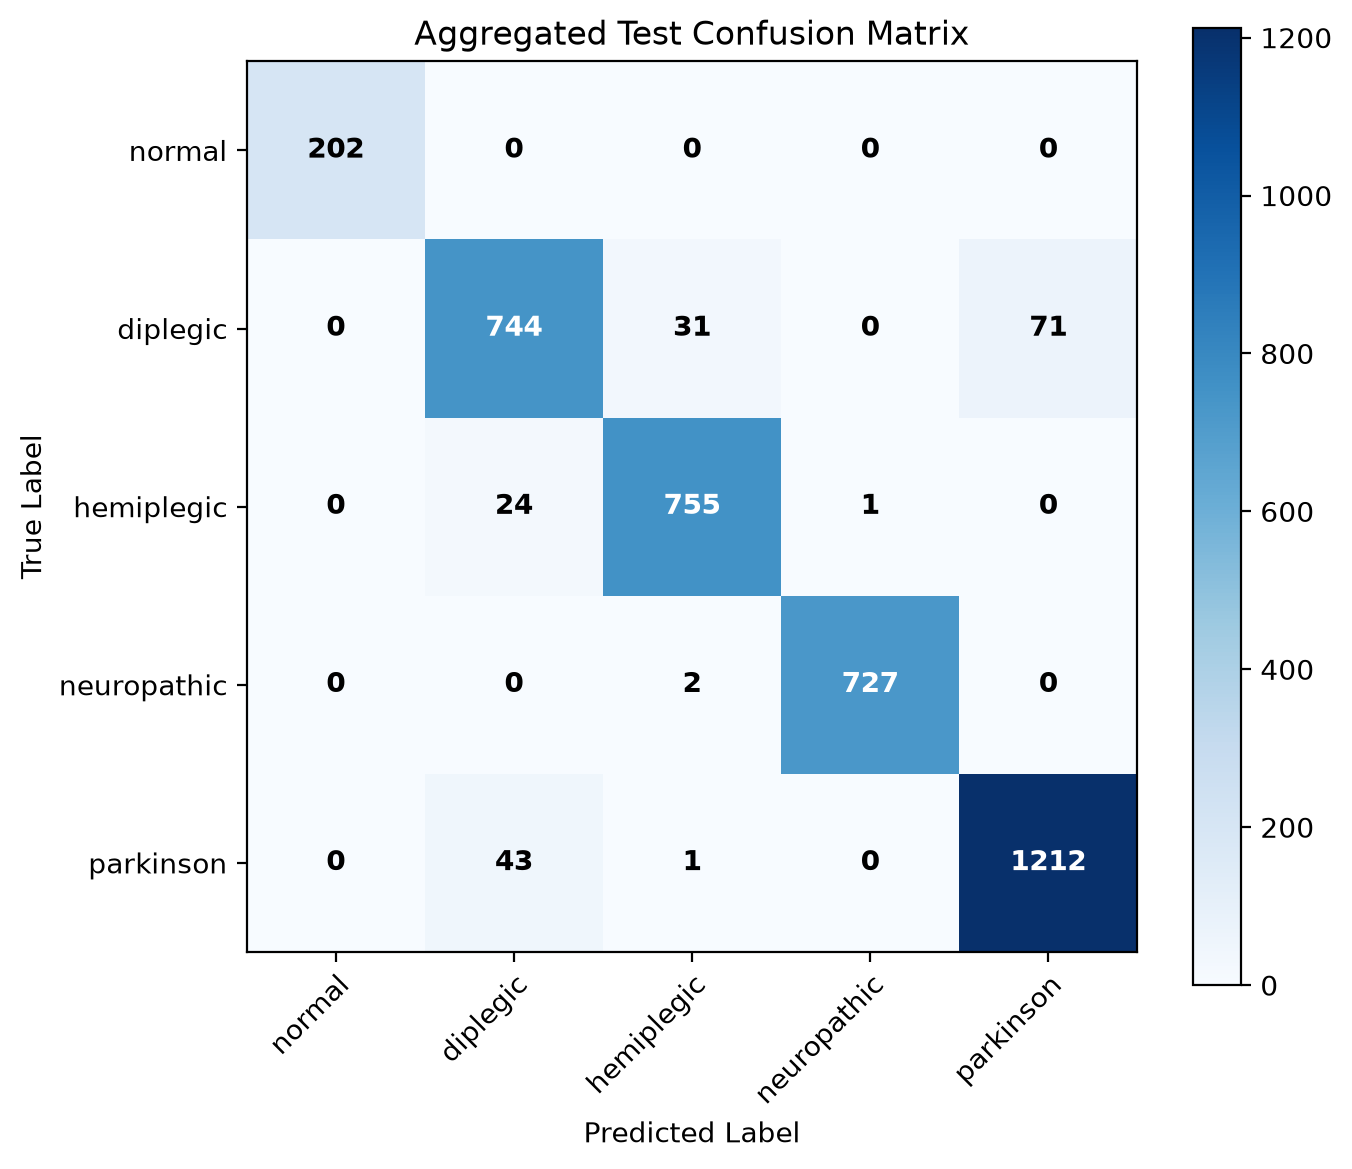
\includegraphics[width=0.495\columnwidth]{cm_gaitit_v6.png}\hfill
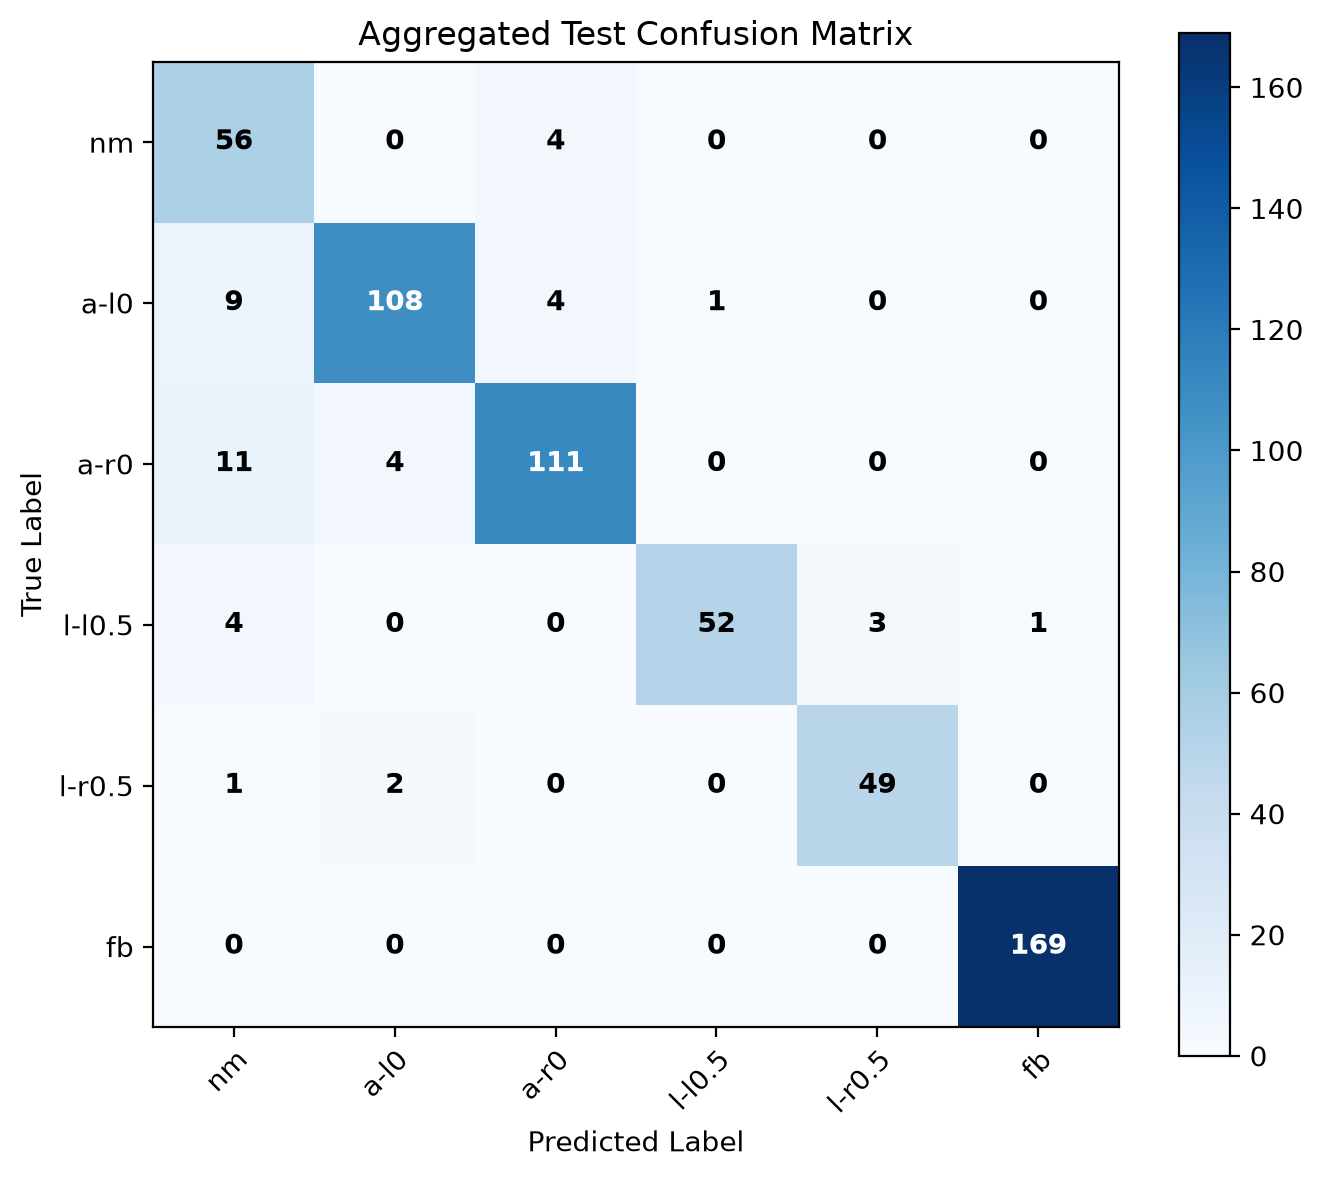
\includegraphics[width=0.495\columnwidth]{cm_init6_v6.png}
\caption{Aggregated test confusion matrices of the final model. Left: GAIT-IT (3813
cycles). Right: INIT, 6 classes (nm: normal; a-l0/a-r0: left/right arm swing
reduced; l-l0.5/l-r0.5: left/right half leg step; fb: full-body impairment).}
\label{fig:cm}
\end{figure}


\begin{figure}[!t]
\centering
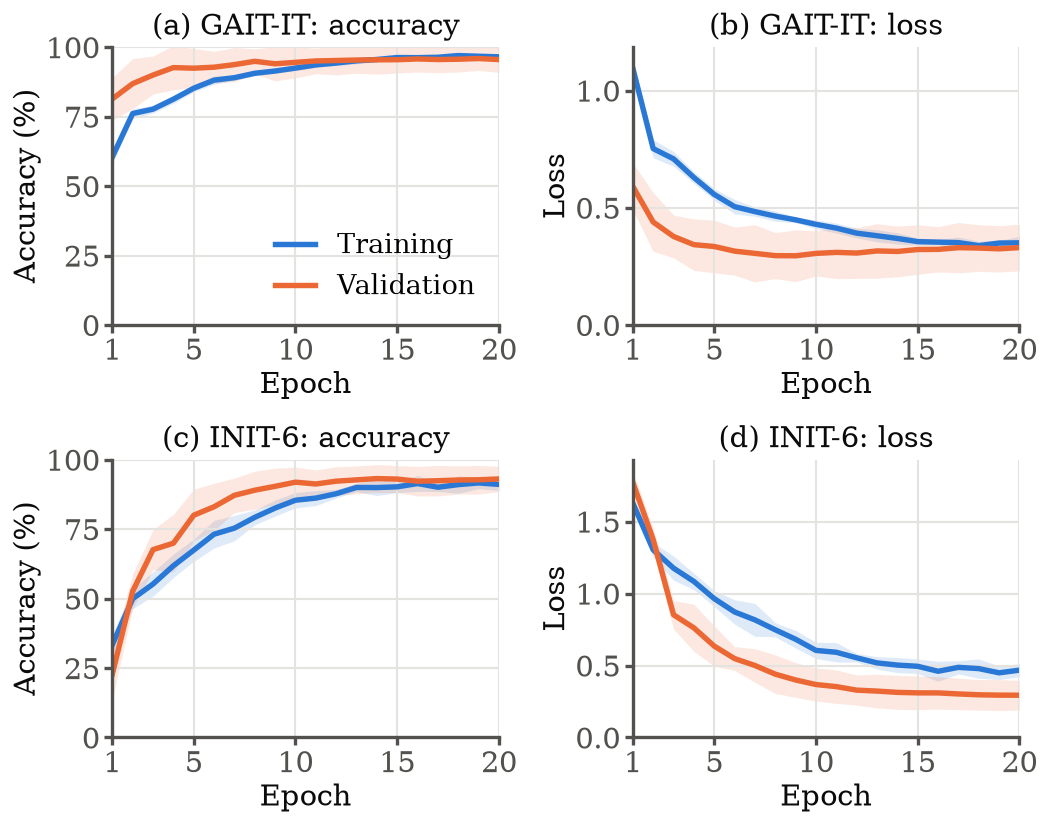
\includegraphics[width=\columnwidth]{curves_v6.png}
\caption{Training and validation accuracy and loss of the final model (EMA
warm-up), mean over 10 folds ($\pm1$ std band); validation subjects are unseen.
Both losses are the cycle cross-entropy.}
\label{fig:curves}
\end{figure}

\textbf{Progress.} The largest steps are phase alignment (ST-PhaseNet,
89.1\,\% on unseen subjects) and anatomical cropping ($+2.3$ points). The
defect fixes mainly made results stable across people (fold std
$5.38\rightarrow4.04$, fold 3 $79.9\rightarrow90.9\,\%$). The final model is
best on every metric with fewer parameters than ST-CRA-Net and Swin (5.0 vs.\ 6.6 and 7.8\,M).
The ST-CRA-Net and Swin scores are not comparable: they share subjects between
training and validation.

\textbf{Ablations.} A 2D ResNet with temporal shift~\cite{lin2019tsm}
matches (2+1)D (94.04 vs.\ 94.05\,\%), so the stage-7 gain comes from B1, B4,
B5 and B7. Geometry (B6) adds 0.66 points and lowers fold std by 0.52.
Subject-adversarial training~\cite{ganin2015} gave no gain.

\textbf{Per class.} Recall is 100 (normal), 99.7 (neuropathic), 96.8
(hemiplegic), 96.5 (Parkinsonian) and 87.9\,\% (diplegic) (Fig.~\ref{fig:cm}).
The main error is diplegic$\leftrightarrow$Parkinsonian: both are bilateral,
symmetric and flexed. Geometry (B6) raised diplegic recall from 84.0 to
87.9\,\%.

\textbf{Subject dependence.} Folds 3 and 9 are weakest in every version
(87.6 and 87.4\,\%; others 96--99\,\%); their errors follow those subjects'
walking style.

\textbf{INIT.} All versions reach 92--94\,\% on 6 classes
(Table~\ref{tab:init}); differences are 1--2 test cycles per fold. Most
errors are reduced arm swing predicted as normal (Fig.~\ref{fig:cm}, right): a
missing arm swing changes only a few pixels. On 8 classes the model reaches
$85.56\pm8.19\,\%$.

\textbf{Training behaviour.} On GAIT-IT, validation accuracy on unseen
subjects reaches 92.6\,\% by epoch 4 and levels off near 95.5\,\%; validation
loss never rises, so there is no overfitting, unlike ST-CRA-Net. Training curves
sit slightly below validation because training inputs are augmented. With plain
EMA, INIT validation stayed near chance until epoch 6 (only $\sim$29 steps per
epoch); an EMA warm-up removes this delay (Fig.~\ref{fig:curves}c) but changes
test accuracy by less than one fold std, so reported results use plain EMA.

\textbf{Limitations.} Both datasets contain \emph{simulated} pathologies, and
all results come from one training seed.

% =====================================================================
\section{Conclusion and Future Work}
% =====================================================================
Over nine stages we moved from frame-level attention networks that memorised
people to AnatoPhaseNet, which reaches 95.47\,\% cycle and 96.28\,\% walk
accuracy on unseen GAIT-IT subjects with 5.0\,M parameters, and 92--93\,\% on
INIT-6. The largest gains came from aligning cycles to clinical phases, from
anatomical cropping and part pooling, and from fixing data and transfer
defects. Next we will run multiple seeds, target the diplegic--Parkinsonian
confusion and the weak folds, and test across datasets.

% =====================================================================
\begin{thebibliography}{99}
\footnotesize
\bibitem{baker2018} J.~M. Baker, ``Gait disorders,'' \emph{Am. J. Med.},
vol.~131, no.~6, pp.~602--607, 2018.
\bibitem{albuquerque2021} P. Albuquerque, J.~P. Machado, T.~T. Verlekar,
P.~L. Correia, and L.~D. Soares, ``Remote gait type classification system using
markerless 2D video,'' \emph{Diagnostics}, vol.~11, no.~10, p.~1824, 2021.
\bibitem{ortells2018} J. Ortells, M.~T. Herrero-Ezquerro, and R.~A. Mollineda,
``Vision-based gait impairment analysis for aided diagnosis,'' \emph{Med. Biol.
Eng. Comput.}, vol.~56, no.~9, pp.~1553--1564, 2018.
\bibitem{bodepu_cranet} D. Bodepu, M.~I. Junaid, S. Madarapu, J.~P. Sahoo, and
S. Ari, ``CRA-Net: Cross reverse attention network for classification of
neuro-degenerative diseases based on gait analysis,'' \emph{Biomed. Signal
Process. Control}, vol.~108, p.~107886, 2025.
\bibitem{verlekar2018} T.~T. Verlekar, P.~L. Correia, and L.~D. Soares,
``Using transfer learning for classification of gait pathologies,'' in
\emph{Proc. IEEE BIBM}, 2018, pp.~2376--2381.
\bibitem{carreira2017i3d} J. Carreira and A. Zisserman, ``Quo vadis, action
recognition? A new model and the Kinetics dataset,'' in \emph{Proc. IEEE CVPR},
2017, pp.~6299--6308.
\bibitem{li2023transgait} K. Li and S. Meng, ``TransGait: Vision transformer
based gait recognition network,'' in \emph{Proc. Int. Conf. Image Process.,
Comput. Vision Mach. Learn. (ICICML)}, 2023, pp.~339--343.
\bibitem{hu2018se} J. Hu, L. Shen, and G. Sun, ``Squeeze-and-excitation
networks,'' in \emph{Proc. IEEE CVPR}, 2018, pp.~7132--7141.
\bibitem{woo2018cbam} S. Woo, J. Park, J.-Y. Lee, and I.~S. Kweon, ``CBAM:
Convolutional block attention module,'' in \emph{Proc. ECCV}, 2018, pp.~3--19.
\bibitem{wang2018nonlocal} X. Wang, R. Girshick, A. Gupta, and K. He,
``Non-local neural networks,'' in \emph{Proc. IEEE CVPR}, 2018, pp.~7794--7803.
\bibitem{guo2021ssan} X. Guo, X. Guo, and Y. Lu, ``SSAN: Separable
self-attention network for video representation learning,'' in \emph{Proc. IEEE
CVPR}, 2021, pp.~12618--12627.
\bibitem{liu2021swin} Z. Liu, Y. Lin, Y. Cao, H. Hu, Y. Wei, Z. Zhang, S. Lin,
and B. Guo, ``Swin transformer: Hierarchical vision transformer using shifted
windows,'' in \emph{Proc. IEEE/CVF ICCV}, 2021, pp.~10012--10022.
\bibitem{tran2018r21d} D. Tran, H. Wang, L. Torresani, J. Ray, Y. LeCun, and
M. Paluri, ``A closer look at spatiotemporal convolutions for action
recognition,'' in \emph{Proc. IEEE CVPR}, 2018, pp.~6450--6459.
\bibitem{lin2019tsm} J. Lin, C. Gan, and S. Han, ``TSM: Temporal shift module
for efficient video understanding,'' in \emph{Proc. IEEE ICCV}, 2019,
pp.~7083--7093.
\bibitem{chao2019gaitset} H. Chao, Y. He, J. Zhang, and J. Feng, ``GaitSet:
Regarding gait as a set for cross-view gait recognition,'' in \emph{Proc.
AAAI}, 2019, pp.~8126--8133.
\bibitem{he2016resnet} K. He, X. Zhang, S. Ren, and J. Sun, ``Deep residual
learning for image recognition,'' in \emph{Proc. IEEE CVPR}, 2016, pp.~770--778.
\bibitem{ganin2015} Y. Ganin and V. Lempitsky, ``Unsupervised domain adaptation
by backpropagation,'' in \emph{Proc. ICML}, 2015, pp.~1180--1189.
\end{thebibliography}

\vspace{4mm}
\noindent\begin{tabular}{@{}l@{}}
\rule{4.5cm}{0.4pt}\\
Signature of Supervisor: [[Supervisor Name]]\\
Date: \rule{2.5cm}{0.4pt}
\end{tabular}

\end{document}
